
\chapter{Dislocations in MAX phases}

\label{chap:dislocations_in_max_phases}
\graphicspath{{dislocations_in_max_phases/Figs/}}






In \autoref{chap:hetero_max_phases} elastic heterogeneity of the unit cell was discussed and the local elastic properties were shown to have a strong dependence on the chemical environment. As discussed in  \autoref{chap:plastic_deformation} and shown in \autoref{chap:peierls_model} the dislocation properties are very sensitive to the elastic properties of a crystal. Thus the elastic heterogeneity is expected to have a strong effect on the dislocations in the MAX phases.

The elastic properties of the different layers of the MAX phases are not in the form of full elastic tensors so the approach taken in \autoref{chap:peierls_model} to use the full strain state cannot be applied. Instead a simplified model, adapted from that presented by \citet{Clegg2006} is used that relies on only simple strains and elastic constants. This model was shown to be in reasonable agreement with experiment across orders of magnitude of the Peierls stress and should be sufficient to show the effects of elastic heterogeneity on the Peierls stress.


\section{Adapted Peierls model}

The lack of a full elastic tensor means that the Peierls model used in this case was adapted from the one published by \cite{Clegg2006}. This works in a similar way to the model described in \autoref{chap:peierls_model} except only the first layer of atoms either side of the slip plane are considered and the only displacements allowed are parallel to the Burgers vector, in analogy with the original Peierls model.

The calculation is at the fundamental level very similar, the energy is still a balance between two energy contributions, the elastic energy in the bonds outside the slip plane and the misalignment energy of those bonds across the slip plane. The peierls stress is then the maximum gradient of the energy changes as the dislocation is displaced. However some details have been changed.


The original model was written to calculate the misalignment energy using the Frenkel approximation, as given in \autoref{eqn:Frenkel_approx}, but the adapted model was extended to use a parametrised $\gamma$-surface to represent the misalignment energies, as represented by the summation
\begin{equation}
\gamma = \sum_{m=1}^{M} C_m \left[ 1 - \cos \left( \frac{2m\pi \phi}{b} \right) \right]\label{eqn:gamma_surface}
\end{equation}
where $\gamma$ is the energy in \si{\joule\per\meter\squared}, $C_m$ are a series of parameters fitted by a least-squares method to a set of energies at different misalignments, $m$ is an integer between 1 and some maximum $M$ which is chosen to be the lowest number that adequately captures the energy profile of the $\gamma$-surface, usually 3, $b$ is the burgers vector and $\phi$ is the misalignment in units of \si{\angstrom}, such that $\phi/b$ defines a sort of fractional misalignment.

The other major alteration is that the model in \cite{Clegg2006} optimises the structure of the dislocation only at the equilibrium position, not at every sampled displacement. The adapted model optimises the structure of the dislocation for every position by searching for the dislocation width that yields the lowest dislocation energy.


The elastic moduli and unit cell geometries, both required for the Peierls model, of the regions of the MAX phase structures have been calculated in \autoref{chap:hetero_max_phases} so the only required input for the model is the misalignment potential in the form of the $\gamma$-surface.

\section{Calculating the \texorpdfstring{$\gamma$}{gamma}-surface}


The density functional theory used the same initial set-up as discussed in \autoref{sec:DFT_method}, based on the equilibrated unit cells with periodic boundary conditions in all directions. To calculate the gamma surfaces a displacement across a plane must be imposed, the simplest way to do this is to maintain the periodic boundary conditions and introduce two opposing stacking faults, this is shown schematically in \autoref{fig:DFT_gamma_surface}. There may be a dependence of the stacking fault energy on the distance between stacking faults, and this must be converged, in practice the lattice parameter of the MAX phases is long enough that only one or two unit cell repeats were necessary.

\begin{figure}
\centering
\captionsetup{width=0.45\textwidth}
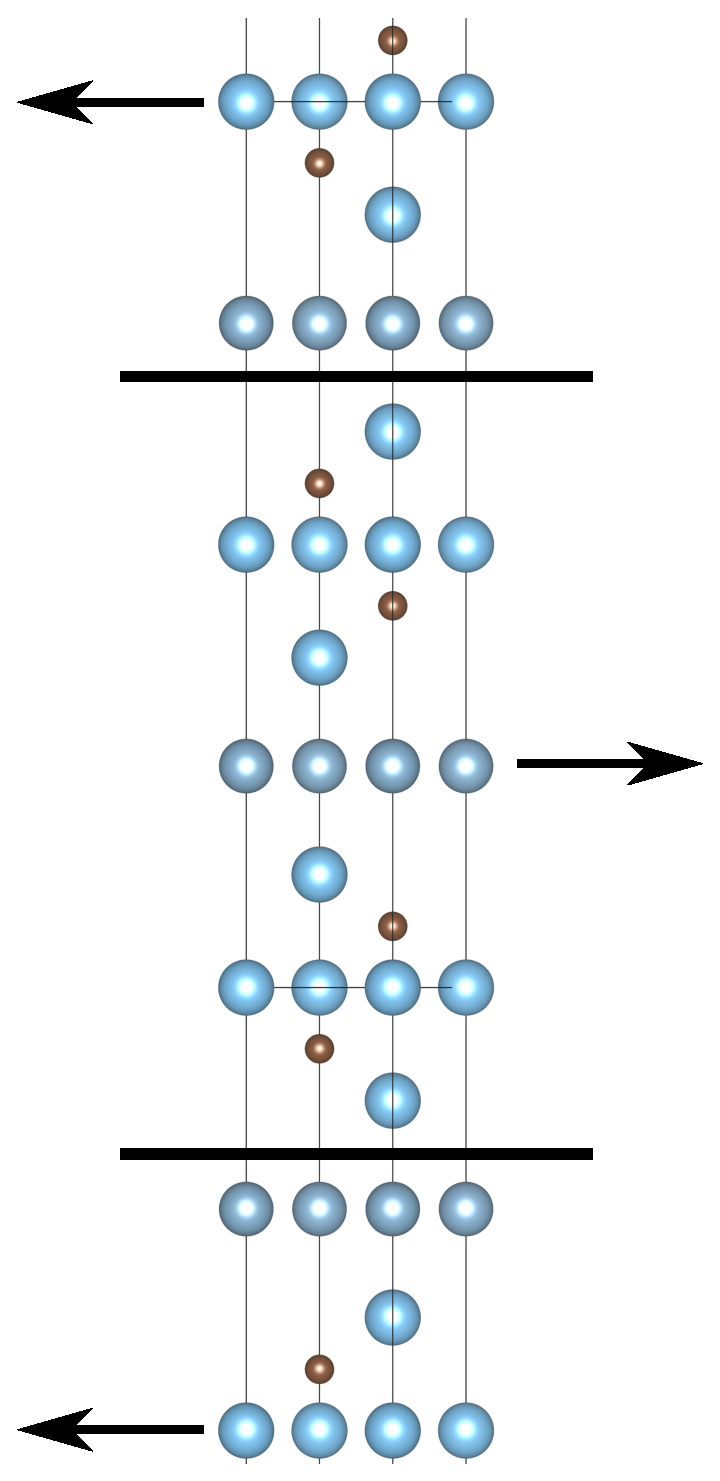
\includegraphics[width=0.3333\textwidth]{displacements_for_gamma_surface}
\caption{Schematic showing the displacements applied to a slab of crystal within a periodic cell. \label{fig:DFT_gamma_surface}}
\end{figure}

To displace the atoms SIESTA's Z-matrix was used \cite{SIESTA_manual}. This allows the coordinates of the atoms to be constrained separately in each direction; the displacement parallel to the slip direction, $a/3$<1\,1\,\={2}\,0> is imposed and the atomic positions are relaxed perpendicular to this displacement. This is important as unreasonably close atomic positions would be imposed without this relaxation. In analogy with the FCC metals it might be expected for there to be a stable stacking fault. The M--A layer can be seen as a single repeat of the HCP structure, with ABA stacking, which their stacking relative to the other M--A layer in the unit cell which is then stacked CBC, see \autoref{fig:MAX_unit_cells}. 

In materials like aluminium dislocations are know to separate into partial dislocation pairs because the stacking fault energy is low enough that dissociating one full dislocation to two partials reduces the overall energy despite the introduction of a stacking fault \cite{kelly2012ch9}. Atoms are therefore displaced along two successive <2\,1\,1> type directions that sum to <1\,0\,1> overall. Even in the case of full dislocations this kind of displacement is likely in the core.

Therefore furthering the analogy with CCP and HCP metals a substantial lateral displacement of atoms is expected. The simplified Peierls model cannot account for this so it must be accounted for during the calculation of the $\gamma$-surface.

Initially 40 samples were taken at even intervals between one perfect position and the next displacing along the <1\,1\,\={2}\,0>. The energy changes, relative to the equilibrium position, were fitted to the function given in \ref{eqn:gamma_surface} using \textttf{scipy.curve_fit} package provided by the SciPy project \cite{SciPy2001}.





\section{Results and discussion}





























